\documentclass[extra]{gji}
\usepackage{timet}

\usepackage{lineno}
\usepackage{float}
\usepackage[fleqn]{amsmath}

\usepackage{mathtools}
\usepackage{graphicx}
\usepackage{url}
\usepackage[utf8x]{inputenc}
\usepackage{booktabs}

% Use abbreviations for references
\newcommand{\equationautorefname}{Eq.}
\newcommand{\tableautorefname}{Tab.}
\newcommand{\figureautorefname}{Fig.}

% Fix line number issue for math environments
\let\oldequation\equation
\let\oldendequation\endequation

\renewenvironment{equation}
  {\linenomathNonumbers\oldequation}
  {\oldendequation\endlinenomath}

\usepackage{xcolor}
\definecolor{darkgray}{gray}{0.5}
\renewcommand{\linenumberfont}{\scriptsize\color{darkgray}}
\definecolor{darkblue}{RGB}{0,0,205}
\usepackage{url}
\usepackage[colorlinks=true]{hyperref}
\hypersetup{
    pdftitle={Quantitative imaging of water, ice, and air in permafrost systems through petrophysical joint inversion of seismic refraction and electrical resistivity data},
    pdfauthor={Florian Wagner (mail@fwagner.info)},
    bookmarks=true,         % show bookmarks bar?
    unicode=false,          % non-Latin characters in Acrobat’s bookmarks
    pdftoolbar=true,        % show Acrobat’s toolbar?
    pdfmenubar=true,        % show Acrobat’s menu?
    pdffitwindow=true,      % page fit to window when opened    ´
    pdfnewwindow=true,      % links in new window
    linkcolor=darkblue,    % color of internal links
    citecolor=darkblue,        % color of links to bibliography
    filecolor=darkblue,      % color of file links
    urlcolor=darkblue,           % color of external links
    bookmarksnumbered=true, %Lesezeichen werden nummeriert dargestellt
    pdfdisplaydoctitle=true,
    pdfstartview=FitV,
}

\begin{document}
\title{Quantitative imaging of water, ice, and air in permafrost systems through petrophysical joint inversion of seismic refraction and electrical resistivity data}
\author[Wagner et al.]{F.M. Wagner$^1$\thanks{\href{mailto:mail@fwagner.info}{mail@fwagner.info}}, C. Mollaret$^2$, T. Günther$^3$, A. Kemna$^1$, C. Hauck$^2$\\
 $^1$ University of Bonn, Institute of Geosciences, Geophysics Section, Bonn, Germany\\
 $^2$ University of Fribourg, Department of Geosciences, Fribourg, Switzerland\\
 $^3$ Leibniz Institute for Applied Geophysics, Hannover, Germany
}

\date{\today}
\pagerange{accepted manuscript (\url{https://doi.org/10.1093/gji/ggz402})}
\volume{}
\pubyear{2019}
\let\leqslant=\leq

\renewcommand{\thefootnote}{\fnsymbol{footnote}}

\maketitle
\begin{summary}
 Quantitative estimation of pore fractions filled with liquid water, ice, and air is crucial for a process-based understanding of permafrost and its hazard potential upon climate-induced degradation.
 Geophysical methods offer opportunities to image distributions of permafrost constituents in a non-invasive manner.
 We present a method to jointly estimate the volumetric fractions of liquid water, ice, air, and the rock matrix from seismic refraction and electrical resistivity data.
 Existing approaches rely on conventional inversions of both data sets and a suitable a-priori estimate of the porosity distribution to transform velocity and resistivity models into estimates for the four-phase system, often leading to non-physical results.
 Based on two synthetic experiments and a field data set from an Alpine permafrost site (Schilthorn, Bernese Alps, Switzerland), it is demonstrated that the developed petrophysical joint inversion provides physically plausible solutions, even in the absence of prior porosity estimates.
 An assessment of the model covariance matrix for the coupled inverse problem reveals remaining petrophysical ambiguities, in particular between ice and rock matrix.
 Incorporation of petrophysical a-priori information is demonstrated by penalizing ice occurrence within the first two meters of the subsurface where the measured borehole temperatures are positive.
 Joint inversion of the field data set reveals a shallow air-rich layer with high porosity on top of a lower-porosity subsurface with laterally varying ice and liquid water contents.
 Non-physical values (e.g., negative saturations) do not occur and estimated ice saturations of 0-50\% as well as liquid water saturations of 15-75\% are in agreement with the relatively warm borehole temperatures between -0.5\,\textdegree C and 3\,\textdegree C.
 The presented method helps to improve quantification of water, ice, and air from geophysical observations.
\end{summary}

\begin{keywords}
 Seismic tomography, Electrical resistivity tomography (ERT), Joint inversion, Inverse theory, Hydrogeophysics.
\end{keywords}

\section{Introduction}
Climate-induced degradation of permafrost can release substantial amounts of soil organic carbon into the atmosphere \citep[e.g.,][]{Schuur2015} and increase the probability of slope failures in Alpine regions \citep[e.g.,][]{Huggel2012}.
Understanding hydrological processes in permafrost systems is crucial to parameterize numerical models that simulate the evolution and potential carbon feedback of terrestrial permafrost as well as to assess the hazard potential of permafrost degradation on a physical basis.

% Why geophyscis?
While borehole information is expensive and limited to discrete locations, geophysical imaging offers opportunities to derive quantitative and non-invasive insights on permafrost characteristics at high spatial and temporal resolution.
Electrical resistivity and acoustic velocity of a medium are sensitive to the phase change of water between its liquid, frozen, and gaseous states.
Electrical resistivity tomography (ERT) and refraction seismic tomography (RST) are thus widely used in cryospheric geophysical applications \citep{Hauck2008}.

% ERT examples
\cite{Hilbich2008} analyzed a 7-year long ERT and borehole temperature monitoring data set at the Schilthorn, Swiss Alps, and characterized both short-term (e.g., seasonal active layer dynamics) and long-term effects (e.g., ground ice degradation as a consequence of the extraordinary hot European summer in 2003).
\cite{Dafflon2016} combined ERT with frequency-domain electromagnetic induction data, core analysis, and digital surface models to estimate the spatial distribution of shallow permafrost in an Alaskan tundra environment.
\cite{Oldenborger2018} imaged changes in unfrozen water content in accordance with temperature measurements alongside airport infrastructure.

% RST examples
While ERT is highly sensitive to unfrozen water content, quantitative estimates of ice from electrical data alone are impeded since ice and air are practically electrical insulators and may not be distinguished from a resistive rock matrix.
Fortunately, air and ice usually differ by an order of magnitude in their acoustic velocities, in addition to velocity changes of up to 2000\,m/s between frozen and unfrozen water \citep{Hilbich2010}, making RST a valuable additional method in cryospheric geophysics \citep[e.g.,][]{Harris1986, Krautblatter2014, Steiner2019}.
For example, \cite{Dou2014} performed seismic measurements in the arctic permafrost region and identified a low velocity zone, which is likely related to partially thawn saline permafrost and in agreement with ERT measurements by \cite{Hubbard2013}.
\cite{Merz2016} used ERT and RST measurements together with other geophysical as well as geotechnical data for a multidisciplinary characterization of an Alpine rock glacier.
The authors combined the insights obtained from the different methods in a qualitative interpretation and concluded that joint inversions of different geophysical data sets offer opportunities for the quantification of permafrost composition in future studies.

To take advantage of the complementary sensitivities of ERT and RST for the quantification of permafrost constituents, \cite{Hauck2011} presented a petrophysical four-phase model (4PM) incorporating estimates of liquid water, ice, and air contents for given separate inversions of electrical and seismic refraction data sets and a preexisting porosity estimate.
\cite{Mewes2017} assessed the resolution capacity of the 4PM, which depends on the individual resolution capacities of ERT and RST, with regard to the estimation of liquid water and ice contents for typical processes in the context of permafrost degradation.
The authors emphasized that artifacts in the individual inversions can impair the physical plausibility of the estimated constituents and potentially lead to misinterpretation.
They further found that smoothness regularization applied to the individual inversions can underestimate the magnitude of changes.
\cite{Pellet2016} improved the 4PM through soil moisture calibration.
Instead of prescribing the porosity, the authors developed an estimate of its distribution based on a three-phase model in the unfrozen part of the subsurface.
They found that one remaining challenge in the application of the 4PM is the possibility of simulated ice occurrence even in regions where it is highly unlikely, highlighting the need for means to impose physical constraints during inversion.
To this end, we present an approach that uses apparent resistivities and seismic traveltimes simultaneously in a petrophysically coupled joint inversion to improve the quantification of permafrost constituents from geophysical observations.

\section{Theory and method}
\subsection{Acoustic and electrical properties of partially frozen ground}

Following \citet{Hauck2011}, it is assumed that permafrost systems comprise the volumetric fractions of the solid rock matrix ($f_\text{r}$) and a pore-filling mixture of liquid water ($f_\text{w}$), ice ($f_\text{i}$), and air ($f_\text{a}$)
%
\begin{equation}\label{eq:sum}
 f_\text{r} + f_\text{w} + f_\text{i} + f_\text{a} = 1.
\end{equation}
%
The volumetric fractions of the solid rock matrix, liquid water, frozen water, and gaseous water or air, are herein referred to as rock, water, ice, and air content, respectively.
This terminology is chosen for the sole reason of brevity noting that both ice and air can represent different physical states of water, whereas the term rock is commonly used for the bulk medium.
We emphasize that treatment of the rock content as a single phase is a simplification particularly favorable for Alpine permafrost, where the fraction of hard rock is much higher compared to shallow arctic permafrost for example.
The latter may exhibit a pronounced and potentially clay-rich soil layer with very different acoustic and electrical properties than competent porous materials at larger depths.

The seismic slowness ($s$) of the four-phase system, i.e., the reciprocal of the seismic P-wave velocity ($v$), is described by a time-averaging equation that sums up the slownesses of the individual components weighted by their respective volumetric fractions \citep[e.g.,][]{Timur1968}
%
\begin{equation}\label{eq:timur}
 s = \frac{1}{v} = \frac{f_\text{w}}{v_\text{w}} + \frac{f_\text{i}}{v_\text{i}} + \frac{f_\text{a}}{v_\text{a}} + \frac{f_\text{r}}{v_\text{r}}.
\end{equation}
%
\autoref{eq:timur} assumes that the medium is isotropic, has a single homogeneous mineralogy, and is at high effective pressure \citep[e.g.,][]{Mavko2009}.
References to alternative approaches better suited for the characterization of permafrost in unconsolidated materials are provided in the discussion.

Under the assumption that electrolytic conduction dominates, a modification of Archie's second law \citep{Archie1942} is used to describe the electrical resistivity of the bulk medium.
As in \cite{Hauck2011}, the porosity $\phi$ in the original form of Archie's second law is expressed in terms of the rock content, i.e., $\phi = 1-f_\text{r}$, while the liquid water saturation is replaced by the ratio of water content and porosity:
%
\begin{equation}\label{eq:archie}
 \rho= \rho_\text{w} (1 - f_\text{r})^{- m} \left(\frac{f_\text{w}}{1 - f_\text{r}}\right)^{-n}.
\end{equation}
%
Assuming prior estimates of porosity, the Archie parameters (cementation exponent $m$ and saturation exponent $n$), pore water resistivity $\rho_\text{w}$, and the velocities of the four constituents, \cite{Hauck2011} used equations (\ref{eq:sum}), (\ref{eq:timur}), and (\ref{eq:archie}) to derive expressions for water, ice, and air contents.
These are then used to transform tomograms of $\rho$ and $s$, obtained through individual inversions of ERT and RST data sets, into estimates of liquid water, ice, and air (\autoref{fig:workflow}a).
The obtained estimates and their physical plausibility depend on the two tomograms and cannot be constrained directly. In the following, we describe a petrophysically coupled joint inversion approach, which uses both data sets to directly estimate the constituents of the four-phase system (\autoref{fig:workflow}b).

\begin{figure}
 \centering
 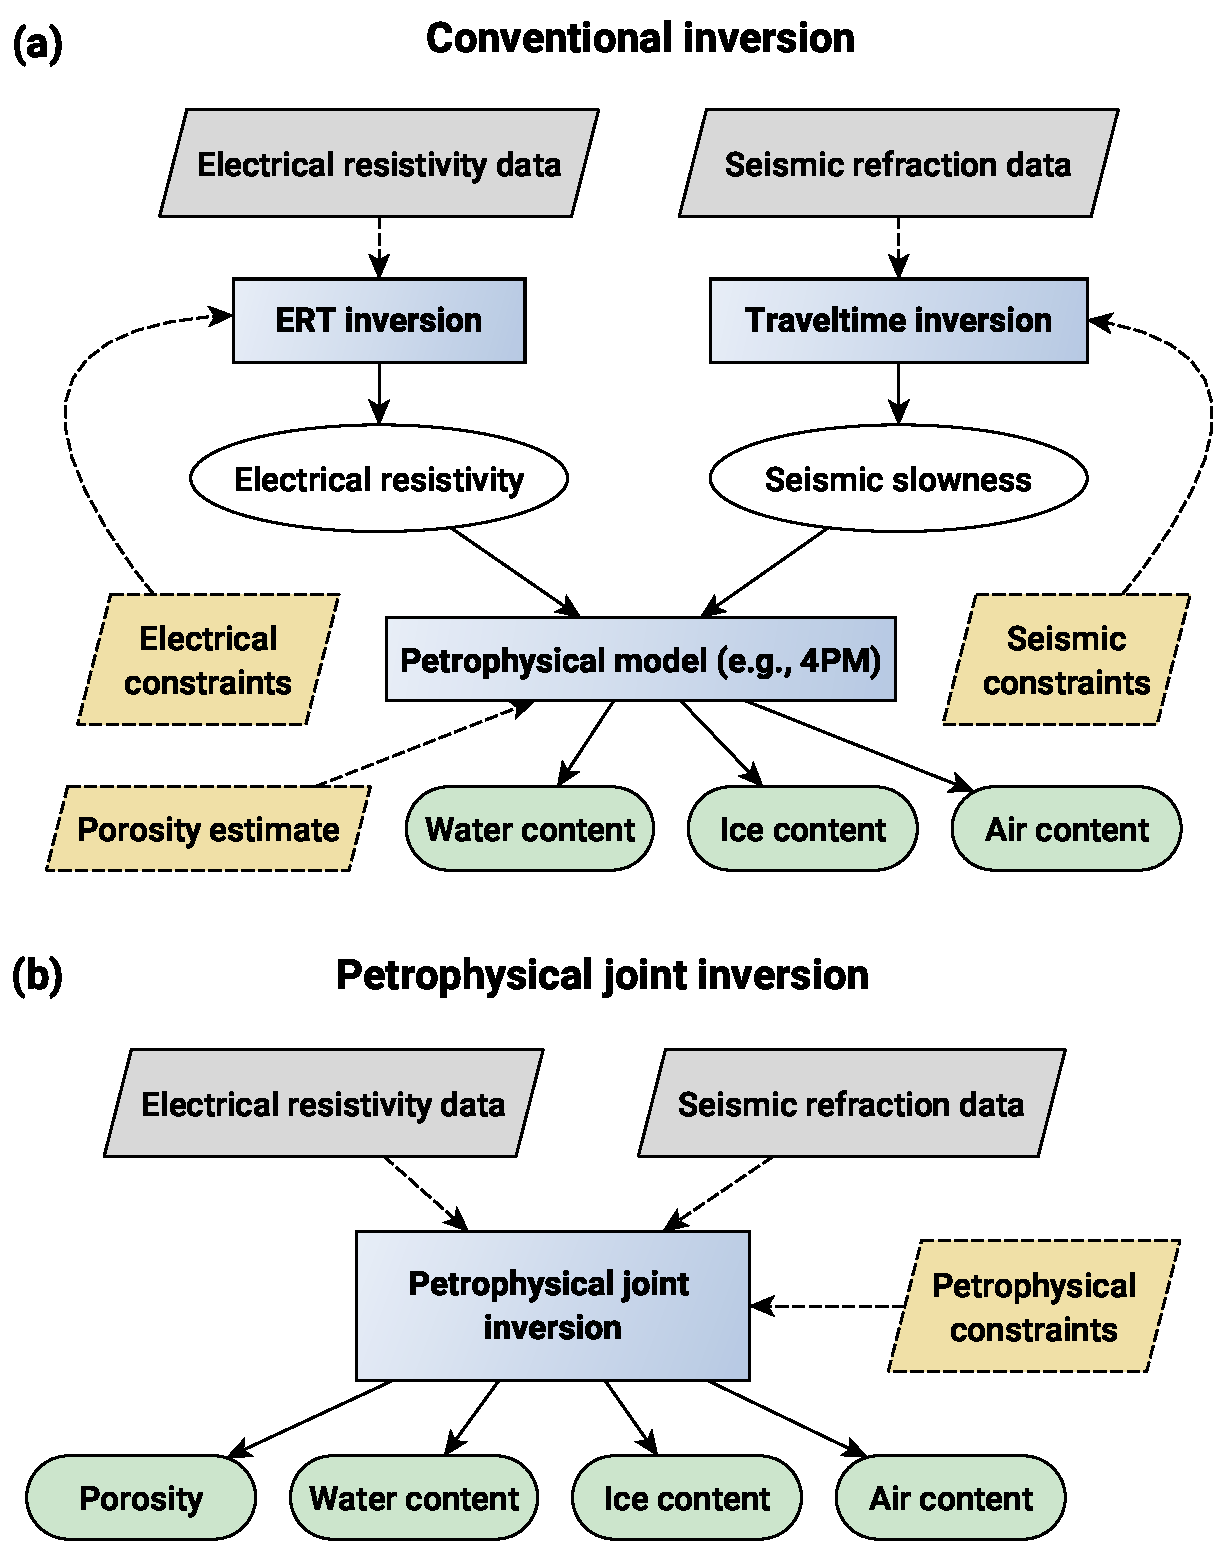
\includegraphics[width=.5\textwidth]{./Fig1_one_column}
 \caption{Schematic on the estimation of water, ice, and air from ERT and RST data.
  (a) Conventional inversion of both data sets with subsequent petrophysical transformation.
  (b) Petrophysical joint inversion honoring both data sets and petrophysical relations during parameter estimation.
 }
 \label{fig:workflow}
\end{figure}

\subsection{Petrophysical joint inversion for permafrost constituents}
The parameter vector $\mitbf{p}$ consists of the volumetric fractions of water, ice, air, and rock for each model cell
%
\begin{equation}\label{eq:model}
 \mitbf{p} = \begin{bmatrix} \mitbf{f}_\text{w} , \mitbf{f}_\text{i} , \mitbf{f}_\text{a} , \mitbf{f}_\text{r} \end{bmatrix}^T.
\end{equation}
%
Theoretically one could only invert for three phases and obtain the fourth one by subtraction from unity, but this would not safeguard against negative values in the fourth phase.
Furthermore, having all four phases in the parameter vector enables flexible incorporation of prior information.
During inversion, a transformed model vector $\mitbf{m}$ is used, where each entry in $\mitbf{p}$ is constrained to vary between zero and one by making use of logarithmic barriers such that $m_j^k = \log(p^k_j) - \log(1 - p^k_j)$ after \citet{KimKim2011}.
The use of logarithmic barriers keeps each volumetric fraction within physical limits (i.e., $0 \leq f_\text{w}, f_\text{i}, f_\text{a}, f_\text{r} \leq 1$) while simultaneously reducing the ill-posedness of the inverse problem.
Here, the indices $j$ and $k$ refer to spatial model cells and type of volumetric pore fraction, respectively.
Traveltimes and logarithmized apparent resistivities are concatenated in the data vector
%
\begin{equation}\label{eq:data}
 \mitbf{d} = \begin{bmatrix} \mitbf{t} , \log(\mitbf{\rho_\text{a}}) \end{bmatrix}^T.
\end{equation}
%
We minimize the following objective function
%
\begin{equation}\label{eq:min}
 \begin{split}
  \| \mitbf{W}_\text{d} (\mitbf{d} - \mathcal{F}(\mitbf{m}) \|^2_2 &+ \alpha^2 \| \mitbf{W}_\text{m} \mitbf{m} \|^2_2\\&+ \beta^2 \| \mitbf{W}^\text{sum}_\text{p}\mitbf{p}-\mitbf{1} \|^2_2\\
  &+ \gamma^2 \| \mitbf{W}_\text{p}(\mitbf{p}-\mitbf{p}_\text{0}) \|^2_2\rightarrow\min.
 \end{split}
\end{equation}

The first term quantifies the misfit between observed data $\mitbf{d}$ and the model response $\mitbf{\mathcal{F}}(\mitbf{m})$ incorporating the reciprocals of the individual data errors on the diagonal of data weighting matrix $\mitbf{W}_\text{d}$.
Note that the model response $\mitbf{\mathcal{F}}(\mitbf{m})$ contains petrophysical transformation according to equations (\ref{eq:timur}) and (\ref{eq:archie}) followed by independent solutions of the RST and ERT forward problems.
The second term represents a smoothness regularization applied to the model vector $\mitbf{m}$, where $\mitbf{W}_\text{m}$ is a block matrix holding four first-order roughness operators on its diagonal to promote smoothness in the distribution of each constituent of the four-phase system.
The third term is an additional regularization term to fulfill the volume conservation constraint in \autoref{eq:sum}.
Here, $\mitbf{W}^\text{sum}_\text{p}$ is a block matrix of four adjacent identity matrices acting on the untransformed petrophysical parameter vector $\mitbf{p}$ to penalize solutions for which the sum of the four volumetric fractions deviates from unity.
The fourth term represents a damping regularization and allows to incorporate a-priori information on the petrophysical target parameters by penalizing deviations from a given reference model $\mitbf{p}_\text{0}$.
Here, $\mitbf{W}_\text{p}$ is a square matrix with either zeros or ones along its diagonal depending on which model parameters are sought to stay close to the reference model $\mitbf{p}_\text{0}$.
The fourth term is optional.
For example, we discuss joint inversion results with and without a prescribed porosity distribution throughout this paper.
The former uses $\gamma = 0$, whereas the latter uses $\gamma = \beta$ and $\mitbf{W}_\text{p} = \text{diag}([\mitbf{0},\mitbf{0},\mitbf{0},\mitbf{I}])$ to penalize solutions for which the rock content distribution deviates from its prior estimate.
The dimensionless factors $\alpha$ and $\beta$ scale the influence of the regularization terms.
$\beta$ is chosen large enough to prohibit non-physical solutions, while $\alpha$ is chosen to fit the data within error bounds.

To minimize the objective function (\autoref{eq:min}), the following augmented system of normal equations is solved for the model parameter update $\Delta \mitbf{m}$ in a least-squares sense using the LSQR algorithm by \cite{Paige1982}:
%
\begin{equation}\label{eq:lsqr}
 \begin{bmatrix}
  \mitbf{W}_\text{d} \hat{\mitbf{J}}        \\
  \alpha \mitbf{W}_\text{m}                 \\
  \beta \hat{\mitbf{W}}^\text{sum}_\text{p} \\
  \gamma \hat{\mitbf{W}}_\text{p}
 \end{bmatrix}
 \Delta \mitbf{m} =
 \begin{bmatrix}
  \mitbf{W}_\text{d} (\mitbf{d} - \mathcal{F}(\mitbf{m}))           \\
  -\alpha \mitbf{W}_\text{m} \mitbf{m}                              \\
  \beta (\mitbf{1} - \hat{\mitbf{W}}^\text{sum}_\text{p} \mitbf{m}) \\
  \gamma (\mitbf{p}_\text{0} - \hat{\mitbf{W}}_\text{p} \mitbf{m})
 \end{bmatrix}.
\end{equation}
%
Due to the use of logarithmic barriers, the transformed parameters $\mitbf{m}$ are a non-linear function of the petrophysical target parameters $\mitbf{p}$.
Since the volume conservation and damping constraints are acting on the latter, the model weighting matrices $\mitbf{W}^\text{sum}_\text{p}$ and $\mitbf{W}_\text{p}$ have to be scaled with the reciprocals of the partial derivative of $\mitbf{m}$ with respect to $\mitbf{p}$ at each iteration before multiplication with the model update $\Delta \mitbf{m}$, i.e., $\hat{\mitbf{W}}_\text{p} = \mitbf{W}_\text{p}\,\text{diag}(\partial m/\partial p)^{-1}$ and $\hat{\mitbf{W}}^\text{sum}_\text{p} = \mitbf{W}^\text{sum}_\text{p}\,\text{diag}(\partial m/\partial p)^{-1}$.
Similarly, the Jacobian matrix $\hat{\mitbf{J}}$ is recomputed at each iteration $\hat{\mitbf{J}} = \mitbf{J}\,\text{diag}(\partial m/\partial p)^{-1}$, where $\mitbf{J}$
holds the changes in traveltime and logarithmic apparent resistivity with respect to changes in the petrophysical target parameters:
%
\begin{equation}\label{eq:jacobian}
 \mitbf{J} =
 \begin{bmatrix}
  \frac{\partial t}{\partial f_\text{w}}                   & \frac{\partial t}{\partial f_\text{i}}                   & \frac{\partial t}{\partial f_\text{a}}                   & \frac{\partial t}{\partial f_\text{r}}                   \\
  \frac{\partial \log(\rho_\text{a})}{\partial f_\text{w}} & \frac{\partial \log(\rho_\text{a})}{\partial f_\text{i}} & \frac{\partial \log(\rho_\text{a})}{\partial f_\text{a}} & \frac{\partial \log(\rho_\text{a})}{\partial f_\text{r}}
 \end{bmatrix}.
\end{equation}
%
The individual matrix entries are obtained by appropriate scaling of the common Jacobian entries of both methods.
Scaling factors are dependent on the underlying petrophysical model (here \autoref{eq:timur} and \autoref{eq:archie}) and detailed in Appendix~\ref{appendix}.
%

\section{Synthetic examples}
\subsection{Synthetic model and data}
To evaluate the performance of the joint inversion approach, a three-layer model is considered (\autoref{fig:known_poro}a).
Parameters are defined in terms of water, ice, air, and rock contents and subsequently transformed into velocity and resistivity distributions for the generation of synthetic data.
The model represents a typical layered scenario encountered in Alpine periglacial environments comprising a 5\,m thick, unfrozen active layer (i.e., the seasonal thaw layer), a 10\,m thick partially thawn layer with laterally changing ice and liquid water contents, and a frozen bedrock underneath.
The porosity is decreasing from 40\,\% to 20\,\% layer-wise with depth.
Velocity and electrical resistivity are calculated according to \autoref{eq:timur} and \autoref{eq:archie} with the parameters listed in \autoref{tab:parameters} and generally increase with depth due to the decreases in liquid water and air contents, combined with increases in ice and rock contents.

While the acoustic velocities of water, ice, and air are agreed upon in the literature, $v_r$ is strongly dependent on the type of rock (or soil).
The chosen value of 5500 m/s may represent a metamorphic rock such as a pyritic paragneiss \citep[e.g.,][]{Draebing2012}.
Common literature values are used for the Archie parameters ($m$ and $n$), whereas the pore water resistivity $\rho_w$ was chosen on the basis of laboratory measurements in an Alpine permafrost context \citep[e.g.,][]{Hauck2008}.
All parameters in \autoref{tab:parameters} are chosen to be constant throughout the model domain and not estimated during inversion.
We refer to \cite{Hauck2011} for a sensitivity analysis of $v_r$, $\rho_w$, $m$ and $n$ in the context of ice estimation.

\begin{table}
 \centering
 \caption{Petrophysical parameters used in \autoref{eq:archie} (left) and constituent velocities used in \autoref{eq:timur} (right) for the synthetic examples. All parameters are assumed to be spatially constant.}
 \begin{tabular}{lrllrl}
  \toprule
  \multicolumn{3}{l}{\textbf{Archie parameters}} & \multicolumn{3}{l}{\textbf{Constituent velocities}} \\ \midrule
  Parameter       & Value & Unit      & Parameter    & Value & Unit \\ \midrule
  $\rho_\text{w}$ & 150   & $\Omega$m & $v_\text{w}$ & 1500  & m/s  \\
  $n$             & 2     & -         & $v_\text{i}$ & 3500  & m/s  \\
  $m$             & 1.3   & -         & $v_\text{a}$ & 330   & m/s  \\
                  &       &           & $v_\text{r}$ & 5500  & m/s  \\
  \bottomrule
 \end{tabular}
 \label{tab:parameters}
\end{table}

Synthetic traveltime data are generated assuming 53 geophones spaced by 2.5\,m and collocated shot positions resulting in 2756 shot-receiver pairs.
Raytracing utilizes the shortest path method with three additional nodes on each edge of a triangular model cell to increase the ray path accuracy following the approach outlined by \cite{Giroux2013}.
Traveltime noise was added as Additive Gaussian White Noise (AGWN) with a standard deviation of 0.5\,ms.

Electrode positions coincide with geophone locations.
A dipole-dipole data set with dipole lengths of one, two, and four unit electrode spacings is simulated neglecting absolute geometric factors above 5000\,m resulting in 1414 apparent resistivities.
Forward modeling employs quadratic shape functions, an enlarged forward modeling domain to avoid boundary effects, and is detailed by \cite{Ruecker2006}.
A normally distributed relative error of 5\,\% was added to the simulated apparent resistivities.
All conventional and joint inversion results presented in the following use four times larger smoothing in the horizontal direction to promote the expected layered structure and describe the synthetic data sets within their respective error bounds.

\subsection{Inversion with correct porosity estimate}

Conventional inversion results of traveltimes and apparent resistivities (\autoref{fig:known_poro}b) are obtained using a Gauss-Newton scheme with smoothness regularization as detailed in \cite{Ruecker2017}.
Velocity and electrical resistivity tomograms are transformed into distributions of water, ice, and air using the 4PM and assuming that the porosity structure is known.

\begin{figure*}
 \centering
 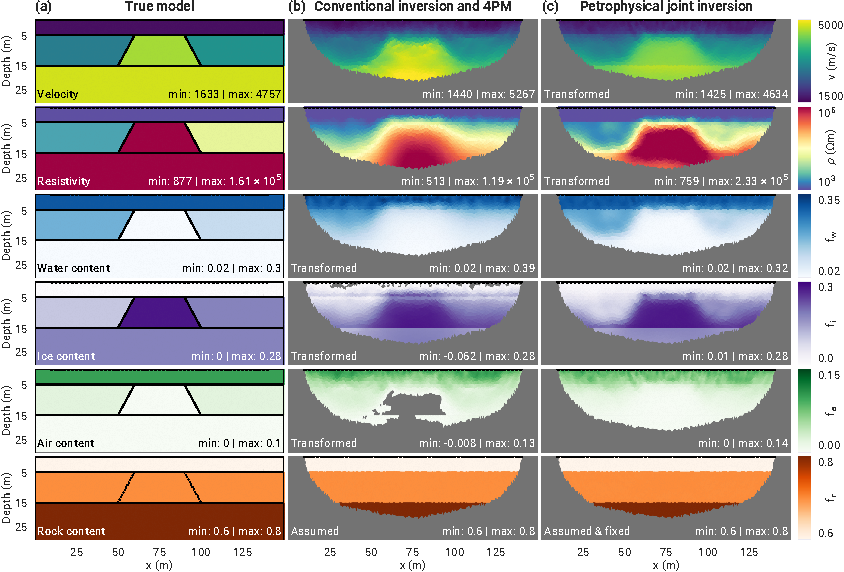
\includegraphics[width=\textwidth]{./Fig2_two_columns}
 \caption{(a) True model, (b) conventional inversion results, and (c) joint inversion results with a-priori knowledge of the porosity distribution. All models are cut off below the lowermost ray path and in regions where the respective volumetric fraction is negative. Sensors are marked as black semicircles. Note that the electrical resistivity (second row) is displayed on a logarithmic color scale. If not otherwise indicated in the lower left of each panel, the distributions shown in (b) and (c) directly result from the respective inversions. The annotation \textit{Transformed} means that the respective quantity is obtained through transformation of the actual inversion results using petrophysical equations.}
 \label{fig:known_poro}
\end{figure*}

The different volumetric fractions are qualitatively and quantitatively in good agreement with the true model.
Solely in the conductive and low velocity top layer, where the individual inversions exhibit small-scale variability close to the sensors, the 4PM produces small regions of negative ice content down to -6\% and overestimates the water content by up to 9\%.

\autoref{fig:known_poro}c shows the results obtained with the developed petrophysical joint inversion approach.
The quantitative agreement to the true model (\autoref{fig:known_poro}a) is slightly better in comparison to the conventional inversion and the layer boundaries are more pronounced.
Moreover, non-physical values do not occur close to the sensors.

\subsection{Inversion with incorrect porosity estimate}

We evaluate the inversion performance without detailed knowledge of the porosity distribution, as common for field applications (\autoref{fig:unknown_poro}).
Note that the true model has not changed, i.e., \autoref{fig:known_poro}a and \autoref{fig:unknown_poro}a show identical distributions.
For the conventional inversion, a homogeneous rock matrix content of 70\,\% (i.e., $\phi = 0.3$) is assumed (lowermost panel in \autoref{fig:unknown_poro}b).
This estimate is correct for the middle layer, but under- and overestimates the porosities of the top and bottom layer by 10\,\%, respectively, leading to non-physical ice content estimations in the top layer (reaching -14\,\%).
In turn, ice contents in the bottom layer are strongly overestimated.
This overestimation stems from the assumption of homogeneous porosity, as the high velocity below 15\,m depth can no longer be explained by a porosity decrease and is compensated by additional ice.
Furthermore, the air content in this region is non-physical (i.e., slightly below zero).

\begin{figure*}
 \centering
 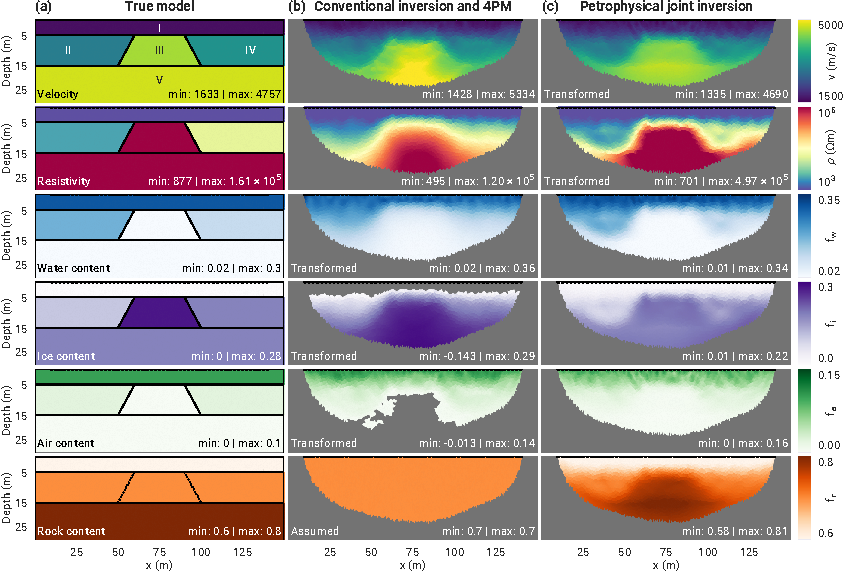
\includegraphics[width=\textwidth]{./Fig3_two_columns}
 \caption{As \autoref{fig:known_poro} but without a-priori knowledge of the porosity distribution.}
 \label{fig:unknown_poro}
\end{figure*}

In the corresponding joint inversions, homogeneous rock content was only used as the starting model for $f_\text{r}$ and allowed to vary by +/- 15\,\% during the inversion.
Estimates of water, ice, and air contents are significantly improved through the joint inversion approach and do not exhibit any non-physical values (\autoref{fig:unknown_poro}c).
Moreover, the inversion indicates a porosity decrease with depth revealing that the measured data cannot be explained with the homogeneous starting model of $f_\text{r}$.
The high ice content in the center of the model cannot be reconstructed and is compensated by an increase in rock content.

\subsection{Model parameter interdependency}
To quantify the interdependency of water, ice, air, and rock content, we consider the model covariance matrix of the coupled inverse problem.
The model covariance elucidates how errors in the data are propagated into errors of the estimated model parameters.
Diagonal elements represent variances of the corresponding parameters, while off-diagonal values indicate correlations between pairs of model parameters \citep[e.g.,][]{Aster2012}.
For better illustration, the parameters are grouped into five discrete blocks as outlined in \autoref{fig:unknown_poro}a.

To highlight the need for petrophysical constraints, we compare the covariances of the coupled inverse problem without (\autoref{fig:cov}a) and with volume conservation constraints (\autoref{fig:cov}b).
In the unconstrained covariance matrix, the air content has the lowest diagonal values, partly due to generally small air contents in the model.
In addition, the velocity of air differs significantly from the other constituent velocities (\autoref{tab:parameters}) leading to its generally good discriminability.
For the remaining fractions, strong off-diagonal elements appear particularly in regions where the amount of unfrozen water is relatively high (parameters i, ii, and iv).
In comparison, the covariances are considerably lower in regions where the water content is low and no air exists (parameters iii and v).
Covariances within one parameter group and between parameter groups are drastically reduced after applying volume conservation constraints in \autoref{eq:sum} (\autoref{fig:cov}b).
Significant variances remain in the upper unfrozen part of the model (parameter i), where sensitivities are generally higher, indicating that errors in the data are more strongly reflected in errors in the model.
In addition, strong variances are visible between ice and rock contents for the other parameters, i.e., at greater depth.

\begin{figure}
 \centering
 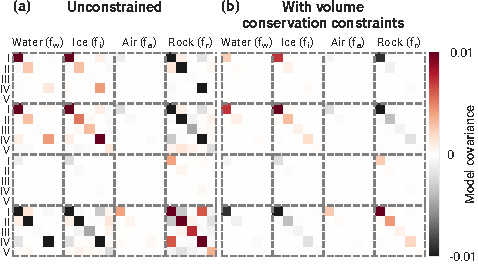
\includegraphics[width=0.5\textwidth]{./Fig4_one_column}
 \caption{Model covariance matrix for the petrophysical joint inversion. Red and black indicate strong positive and negative parameter covariance, white indicates no correlation. The Roman numbering of the model parameters is depicted in \autoref{fig:unknown_poro}a.}
 \label{fig:cov}
\end{figure}

\section{Field data example}

To demonstrate the applicability of the developed joint inversion approach to a real permafrost scenario, we consider a data set acquired at the Schilthorn site located in the Bernese Alps in Switzerland.
The lithology of the Schilthorn massif mainly consists of ferruginous sandstone schists \citep{Imhof2000}.
The bedrock weathering produced a fine-grained surface debris layer with a thickness up to 5 m \citep{Hilbich2008}.
As part of the PACE project, a drilling campaign and first RST and ERT measurements were performed in 1998 to assess the presence of permafrost \citep{VonderMuehll2000}.
Borehole temperature measurements revealed warm permafrost, i.e., near sub-zero temperature, where the liquid water content can be relatively high.
The Schilthorn site became a reference monitoring site of PERMOS \citep[Swiss Permafrost Monitoring Network,][]{permos2016} including numerous measurements of temperature in three boreholes, ground surface temperature, soil moisture, ERT, RST, snow thickness, wind speed and direction, as well as solar radiation.

An ERT monitoring profile was initiated in 1999, automatized in 2009, extended in 2012, and is still maintained and functional \citep[for data acquisition and preprocessing details see][]{Hilbich2008,Hilbich2011,Mollaret2018}.
The ERT acquisition system is composed of 49 fixed electrodes spaced by 2\,m connected to a GeoTom device (GEOLOG, Germany) used with a Wenner configuration.
We only consider the first half of this permanent profile, where collocated geophone positions exist to ensure equal lateral coverage of both methods.
The seismic signal is generated by a sledge hammer striking a steel plate at 25 shot positions located in between each geophone and recorded through a Geode device (Geometrics, USA).
First breaks were manually picked and seismic traveltime errors were estimated to range between 0.1 and 0.5\,ms \citep{Hilbich2010}.
We use 0.3\,ms as an error estimate for the RST data and 3\% relative error for the ERT data.
Similarly as for the inversion of synthetic data, all conventional and joint inversion results use four times larger smoothing in the horizontal direction to promote layered subsurface structures.

We consider a data set measured on August 19, 2014 presented by \cite{Pellet2016}.
On that day, the thaw layer depth in the two boreholes available along the profile was observed around 2.1\,m depth.
In warm recent years, maximum thaw depths at the end of summer reached 9 to 10\,m indicative of considerable permafrost degradation \citep{Permos2019}.
\autoref{fig:schinv}a shows the conventional inversion results with a subsequent application of the 4PM using the parameters from \cite{Pellet2016} as listed in \autoref{tab:parameters_field} and a constant porosity of 53\% based on in-situ measurements performed by \citep{Scherler2006}.
To allow comparability with previous Schilthorn studies \citep[e.g.,][]{Hilbich2008,Pellet2016}, water, ice, and air contents are displayed as saturations, i.e. divided by porosity.

\begin{figure*}
 \centering
 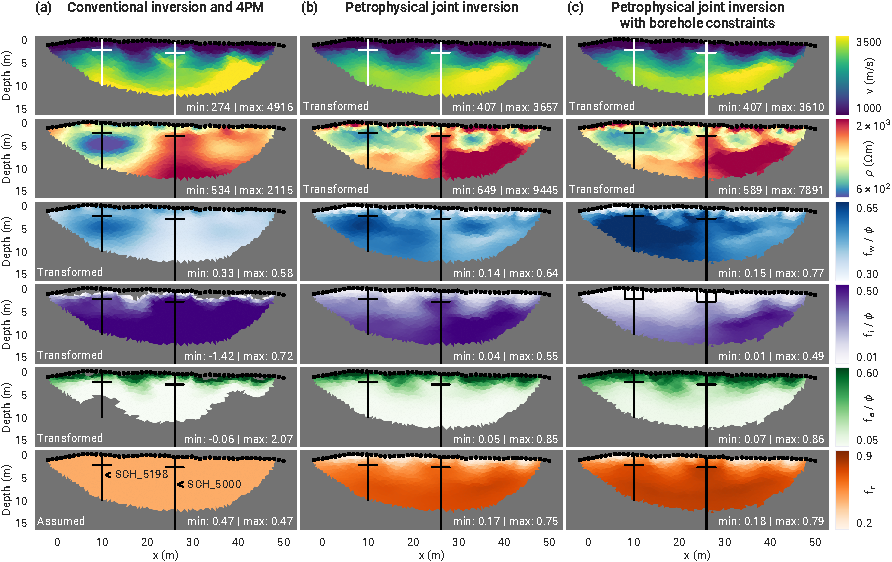
\includegraphics[width=\textwidth]{./Fig5_two_columns}
 \caption{Tomograms of the Schilthorn field data sets obtained through (a) conventional inversion, (b) joint inversion, and (c) joint inversion with borehole constraints. If not otherwise indicated in the lower left of each panel, the shown distributions directly result from the respective inversions.
 All models are cut off below the lowermost ray path and in regions where the respective saturation is negative or exceeds one. Sensors are marked as black circles. Note that the electrical resistivity (second row) is displayed on a logarithmic color scale. Boreholes and associated thaw depths are marked as vertical and horizontal lines, respectively. The black boxes superimposed on the ice saturation in (c) mark the regions where the ice content has been constrained to zero.}
 \label{fig:schinv}
\end{figure*}

\begin{table}
 \centering
 \caption{Petrophysical parameters used in \autoref{eq:archie} (left) and constituent velocities used in \autoref{eq:timur} (right) for the field data example taken from \cite{Pellet2016}. All parameters are assumed to be spatially constant.}
 \begin{tabular}{lrllrl}
  \toprule
  \multicolumn{3}{l}{\textbf{Archie parameters}} & \multicolumn{3}{l}{\textbf{Constituent velocities}} \\ \midrule
  Parameter       & Value & Unit      & Parameter    & Value & Unit \\ \midrule
  $\rho_\text{w}$ & 60    & $\Omega$m & $v_\text{w}$ & 1500  & m/s  \\
  $n$             & 2.4   & -         & $v_\text{i}$ & 3500  & m/s  \\
  $m$             & 1.4   & -         & $v_\text{a}$ & 300   & m/s  \\
                  &       &           & $v_\text{r}$ & 6000  & m/s  \\
  \bottomrule
 \end{tabular}
 \label{tab:parameters_field}
\end{table}

With a prescribed and constant porosity, the conventional approach can only satisfy the low velocities near the surface with non-physical values for ice and air saturations reaching -142 and +207\%, respectively (\autoref{fig:schinv}a).
In contrast, non-physical values do not occur in the petrophysical joint inversion results, as lower porosities near the surface (\autoref{fig:schinv}b) are allowed during parameter estimation.

Since the joint inversion is formulated in terms of the petrophysical target parameters, it becomes possible to include prior information, e.g., constraints on water content based on soil moisture measurements or temperature-dependent constraints on ice occurrence.
Here, we demonstrate the latter by constraining ice contents to zero, where the measured borehole  temperatures (shown in Fig. \ref{fig:sch5198}a and \ref{fig:sch5000}a) are positive.
This is achieved by creating a box with a radius of 2\,m around the corresponding depth interval of the borehole (as indicated for ice saturation in \autoref{fig:schinv}c) and adding cells in this box to the damping constraint in \autoref{eq:min}.
To allow for sharp transitions in the vertical direction across the known thaw depth, we disable smoothing regularization across the lower boundary of this box (by setting the corresponding entries of $\mitbf{W}_\text{m}$ to zero).
A similar approach has been used by \cite{Wunderlich2018} to constrain ERT inversion results to direct push electrical conductivity logs.

While generally comparable to the unconstrained version (\autoref{fig:schinv}b), no ice appears in the upper two meters around the boreholes in the joint inversion result with borehole constraints (\autoref{fig:schinv}c).
The decrease in ice also affects deeper parts of the model and is compensated by an increase in rock content (i.e., a decrease in porosity), which in turn leads to higher water saturations.
The air saturation in all three approaches is high in the thawed part of the model and quickly approaches zero at larger depths.

\begin{figure*}
 \centering
 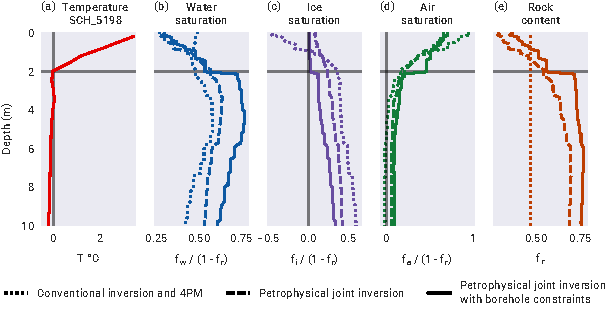
\includegraphics[width=.75\textwidth]{./Fig6_two_columns}
 \caption{(a) Temperature measured on August 19, 2014 in borehole SCH\_5198 and (b-e) corresponding four-phase constituents derived from conventional inversion and petrophysical joint inversion without and with borehole constraints. The horizontal and vertical gray lines mark the thaw depth and zero line, respectively. The borehole location is depicted in the lower left panel of \autoref{fig:schinv}.}
 \label{fig:sch5198}
\end{figure*}

\begin{figure*}
 \centering
 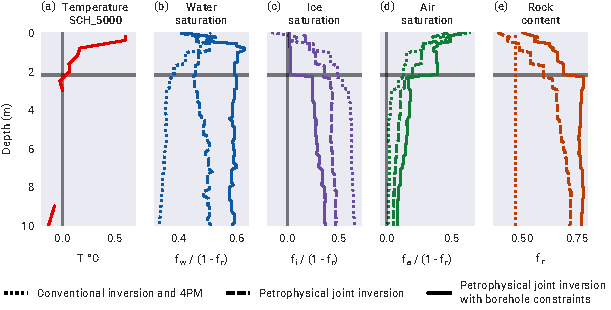
\includegraphics[width=.75\textwidth]{./Fig7_two_columns}
 \caption{(a) Temperature measured on August 19, 2014 in borehole SCH\_5000 and (b-e) corresponding four-phase constituents derived from conventional inversion and petrophysical joint inversion without and with borehole constraints. The horizontal and vertical gray lines mark the thaw depth and zero line, respectively. The borehole location is depicted in the lower left panel of \autoref{fig:schinv}.}
 \label{fig:sch5000}
\end{figure*}

To highlight quantitative differences between the different inversion approaches, \autoref{fig:sch5198} and \autoref{fig:sch5000} show the measured borehole temperatures with depth together with the inversion results shown in \autoref{fig:schinv} extracted at the borehole locations.
The effect of logarithmic barriers can be seen in \autoref{fig:sch5198}c for instance, where in contrast to the conventional approach, joint inversion results do not cross the zero line.

While the conventional inversion and joint inversion without borehole constraints show smooth transitions of ice saturation in the upper few meters for example, the added borehole constraints result in sharp transitions, i.e., a better delineation of the thawn layer (e.g., \autoref{fig:sch5000}c).
Again, it can be seen how the decrease in ice (e.g., \autoref{fig:sch5000}c) is causing an increase in rock content (e.g., \autoref{fig:sch5000}e), which in turn increases water saturation (e.g., \autoref{fig:sch5000}b).

\section{Discussion}
Transformation of conventionally inverted velocity and resistivity tomograms into estimates of water, ice, and air can lead to non-physical results in the presence of data errors and incorrect porosity estimates.
For the Schilthorn case, this was also found by \cite{Pellet2016}, who then derived porosity in the unfrozen part from a three-phase model calibrated to shallow soil moisture measurements and assumed a gradient porosity in the deeper part.
With the assumption of porosity decrease with depth and soil moisture measurements, \cite{Pellet2016} obtained tomograms comparable to our results from the petrophysical joint inversion, which used no prior information on porosity.

Petrophysical joint inversion combines the information of RST and ERT measurements and leads to quantitatively improved images by honoring petrophysical relations and volume conservation during parameter estimation.
Inversion of synthetic data without a porosity estimate (\autoref{fig:unknown_poro}c) and analysis of the model covariances has revealed a strong ambiguity between ice and rock contents.
This ambiguity also became apparent in the application to field data and is in agreement with the findings by \cite{Hauck2011}.
The authors analytically explored the range of possible values for ice, water, air, and rock contents for a given pair of resistivity and velocity values.
By comparing the spread of solutions, it was found that air and water content can be discriminated quite well even if porosity is unknown, while there is a strong ambiguity between ice and rock contents.

The discriminability between ice and rock matrix could be improved by incorporation of additional freeze-thaw sensitive data sets such as complex electrical resistivity measurements.
Results of first laboratory \citep{Wu2013, Kemna2014} and field studies \citep{Grimm2015, Mudler2019} hold promise for ice quantification, as the spectral response of frozen ground is strongly affected by the electrical polarization characteristics of ice.
Ambiguity could further be reduced in a monitoring context, where the porosity can be assumed to be constant within the observed period \citep{Hauck2017}.
Inclusion of multiple timesteps into a time-lapse joint inversion therefore represents a promising extension to this work.

The approach presented is not restricted to the empirical model by \cite{Archie1942} and the time-averaging equation by \cite{Timur1968} and does not attempt to address their general shortcomings.
For example, a general and often overlooked problem is that the empirical factors (e.g., the saturation exponent) are commonly assumed to be spatially constant in field applications.
Future extensions of our work could incorporate advanced petrophysical formulations more representative for the studied field sites.

For the case of saline permafrost for example, \cite{Wu2017} presented a modified formulation, which takes structural soil changes as well as temperature-dependent salinity changes (i.e., electrical conductivity changes) of unfrozen water during freeze-thaw transitions into account.
Based on a field survey on a rock glacier and associated laboratory measurements, \cite{Duvillard2018} emphasized that surface conduction can be significant and has to be taken into account when estimating liquid water content in environments where electrolytic conduction is not dominating the bulk electrical conductivity.
For the case of low-porosity hard rocks, \cite{Draebing2012} presented a modified Timur equation that accounts for changes in matrix velocity due to ice pressure.
\cite{Dou2017} presented a two-end-member mixing approach accounting for the coexistence of frame-strengthening and pore-filling ice to describe the P-wave velocity in saturated, unconsolidated saline permafrost, where conventional slowness averaging would be inadequate.

\section{Conclusions}
We have developed a petrophysical joint inversion approach that uses seismic traveltimes and apparent resistivities to image distributions of water, ice, air, and rock content.
Since petrophysical relations and volume conservation are honored during parameter estimation, our approach produces physically meaningful results, even in the absence of correct porosity estimates, and thereby outperforms post-inversion transformation of conventional tomograms.
A significant advantage is that the inversion constraints can be formulated in terms of the petrophysical target parameters facilitating the flexible use of a-priori information and direct incorporation of non-geophysical data, e.g., constraints on water content inferred from soil moisture measurements, into the inversion.

An application to a field data set from the Schilthorn, Swiss Alps, has revealed physically plausible tomograms in agreement with previous studies without relying on suitable a-priori porosity estimates.
We conclude that our method contributes to improved quantification of water, ice, and air from geophysical observations and will therefore be of direct use for researchers and practitioners in cryogeophysical and hydrogeophysical applications.

Yet joint inversion alone is not able to overcome the inherent petrophysical ambiguities between ice and rock matrix, which remain to be addressed in future studies through additional (non-)geophysical observations, advanced petrophysical formulations, and monitoring applications.
To facilitate adoption and further development of the method, we made the algorithm available under a permissive BSD license.
It is based on the open-source modeling and inversion library \textit{pyGIMLi} \citep{Ruecker2017}.
The implementation as well as scripts to reproduce results and figures of this paper can be found at \url{https://github.com/florian-wagner/four-phase-inversion}.

\begin{acknowledgments}
 The first author gratefully acknowledges funding received by the Dr. Erich Ritter foundation in cooperation with the Water Science Alliance, which allowed preparation of this article during a research visit at Lawrence Berkeley National Laboratory inspired by many fruitful discussions with colleagues in the Earth and Environmental Sciences Area.
 The constructive comments by editor J\"org Renner, Adam Booth and three anonymous reviewers helped to improve earlier versions of this manuscript.
\end{acknowledgments}

\bibliographystyle{gji}
\bibliography{references}

\appendix
\section{Petrophysically transformed Jacobian}\label{appendix}
Changes in traveltime and apparent resistivity with respect to changes in the petrophysical target parameters are obtained by chain rule splitting, where the outer derivative represents the common Jacobian entries of both methods, i.e., $\partial t/\partial s$ and $\partial \log(\rho_\text{a})/\partial \log(\rho)$, whereas the inner derivative applies appropriate petrophysical scaling according to equations (\ref{eq:timur}) and (\ref{eq:archie}).
Additional multiplication with $\rho/\rho_\text{a}$ accounts for the logarithmic transform used in the Jacobian entries of the conventional geoelectrical inverse problem.

\begingroup
\renewcommand*{\arraystretch}{1.5}
\begin{equation}\label{eq:jacfull}
 \begin{split}
  \mitbf{J} &=
  \begin{bmatrix*}[c]
   \frac{\partial t}{\partial f_\text{w}} & \frac{\partial t}{\partial f_\text{i}} & \frac{\partial t}{\partial f_\text{a}} & \frac{\partial t}{\partial f_\text{r}}\\
   \frac{\partial \log(\rho_\text{a})}{\partial f_\text{w}} & \frac{\partial \log(\rho_\text{a})}{\partial f_\text{i}} & \frac{\partial \log(\rho_\text{a})}{\partial f_\text{a}} & \frac{\partial \log(\rho_\text{a})}{\partial f_\text{r}}
  \end{bmatrix*}
  \\&=
  \begin{bmatrix*}[r]
   \frac{\partial t}{\partial s}\frac{\partial s}{\partial f_\text{w}} & \frac{\partial t}{\partial s}\frac{\partial s}{\partial f_\text{i}} & \frac{\partial t}{\partial s}\frac{\partial s}{\partial f_\text{a}} & \frac{\partial t}{\partial s}\frac{\partial s}{\partial f_\text{r}} \\
   \frac{\rho}{\rho_\text{a}}\frac{\partial \rho_\text{a}}{\partial \rho}\frac{\partial \rho}{\partial f_\text{w}} & \frac{\rho}{\rho_\text{a}}\frac{\partial \rho_\text{a}}{\partial \rho}\frac{\partial \rho}{\partial f_\text{i}} & \frac{\rho}{\rho_\text{a}}\frac{\partial \rho_\text{a}}{\partial \rho}\frac{\partial \rho}{\partial f_\text{a}} & \frac{\rho}{\rho_\text{a}}\frac{\partial \rho_\text{a}}{\partial \rho}\frac{\partial \rho}{\partial f_\text{r}}
  \end{bmatrix*}
  \\&=
  \begin{bmatrix*}[c]
   \frac{\partial t}{\partial s}\frac{1}{v_\text{w}} & \frac{\partial t}{\partial s}\frac{1}{v_\text{i}} & \frac{\partial t}{\partial s}\frac{1}{v_\text{a}} & \frac{\partial t}{\partial s}\frac{1}{v_\text{r}} \\
   -\frac{\rho}{\rho_\text{a}}\frac{\partial \rho_\text{a}}{\partial \rho}\frac{n}{f_\text{w}}\rho & 0 & 0 & \frac{\rho}{\rho_\text{a}}\frac{\partial \rho_\text{a}}{\partial \rho}\left(\frac{m - n}{1 - f_\text{r}}\right)\rho
  \end{bmatrix*}
 \end{split}
\end{equation}
\endgroup

\end{document}
